% =============================================================================
% DN-SC - results section (version 0.4 decoder, hierarchical drift stream, six seeds)
% Every number below is taken from results/gpt2_v0.4_six_seeds (tables/*.csv,
% stream/*.json); none is typed from memory. Figure: fig_primary_endpoint.pdf.
% Requires \usepackage{graphicx} and \usepackage{url} (or hyperref). Adjust \section/\subsection levels and labels
% to the manuscript.
%
% NUMBERS FOR THE ABSTRACT (one sentence, ready to paste):
%   On a hierarchical drift stream with a frozen GPT-2 prior, DN-SC reaches 90%
%   token accuracy with 23.3% fewer real channel symbols per token than a frozen
%   fixed-rate receiver using the same decoder, the return-link signalling of
%   refinement included (27.9% [95% CI 21.6-31.7%] when every audited message is
%   decoded free-running; lower cost on all six seeds, p = 0.031).
%
% NUMBERS FOR THE CONCLUSION:
%   memories alone (fixed rate): 15.5% teacher-forced / 21.2% decoded for real;
%   refinement on top: a further 9.3% / 8.4%; return-link signalling 1.4 bits per
%   token over 2.8 rounds per message; shipped adaptation pays only above about
%   1,000 messages per adaptation step (6,000 relative to the context memory).
%
% REMOVE from the manuscript every number of the earlier pilot that is not
% reproduced here, in particular: "47.7 %", "half the channel symbols", "20.9 %",
% the 71/22/7 % decomposition, and any claim that refinement supplies most of
% the gain or that shipping costs nothing; those figures were teacher-forced,
% without the return-link signalling and with the earlier decoder.
% =============================================================================

\section{Results}
\label{sec:results}

\subsection{Protocol}
\label{sec:results-protocol}

All results use GPT-2 (124M parameters) as the frozen language prior and the
nested codebook of Section~X (16 real channel symbols per token, nested at
2/4/6/8/12/16). The hierarchical drift stream alternates AG News and TeleQnA
(600 adaptation steps of six parallel conversations, topic switch every 30
steps), over an AWGN channel whose SNR follows a clipped AR(1) process with a
mean of 10\,dB. Every message is scored prequentially, with the parameters the
receiver holds before any update. The cost measure is the number of real
channel symbols per token needed for 90\,\% token accuracy, read off each
receiver's measured accuracy--symbols curve.

\emph{Decoder.} Selective refinement uses beam search of width~4 (sentences
ranked by their joint posterior), a first round of 6~symbols per token, and no
reopening of closed tokens. This decoder was chosen on validation text only,
by a rule fixed in advance, among first rounds of 2, 4 and 6~symbols, with and
without reopening, and greedy or beam decoding of width 2 or~4. On the
validation set it needs 8.31 symbols per token with signalling against 8.97
for greedy decoding from 2~symbols. Every fixed-rate reference is decoded with
the same beam, which lowers its own cost by 17.7\,\% (from 10.99 to 9.05
symbols per token); all comparisons below are therefore against the stronger
baseline.

\emph{Signalling.} After every round the receiver tells the transmitter which
tokens to continue. This return-link signalling is charged to selective
refinement at the capacity of the mean SNR, either at the empirical entropy of
the decisions (main figures) or as an explicit bitmap.

\emph{Teacher-forced and real decoding.} The policy is evaluated teacher-forced
on all 600 steps. In addition, every 23rd step (26 steps, 156 messages per run)
the same received symbols are decoded for real, free-running and round by
round, for selective refinement and for every fixed prefix alike. By the
decision rule fixed in advance, the teacher-forced curves are the measurement
if, on the audited steps, real decoding needs at most 5\,\% more forward
symbols than the teacher-forced estimate for every receiver; otherwise the
real-decoding figures replace them. The gap is $+3.4$\,\% (context memory),
$+3.6$\,\% (DN-SC) and $+5.0$\,\% (frozen receiver), so the teacher-forced
figures are the measurement and the real-decoding figures are reported next to
them. (With the earlier greedy decoder from 2~symbols this gap was
27--34\,\%.)

\emph{Seeds and statistics.} The frozen receiver and DN-SC were run on six
seeds (0--5), the context-only receiver on four (0, 3, 4, 5). Seeds 0--2 ran
on a Linux CPU and seeds 3--5, which had never been run before, on a Windows
laptop CPU, with the same code and the same codebook. Real-decoding intervals
are 95\,\% percentile intervals from 2000 paired bootstrap draws of the audited
steps within each seed. The seed-level test is an exact sign-flip permutation
test on the per-seed costs; with six seeds its smallest attainable $p$-value
is $2/2^6 = 0.031$.

\subsection{Primary endpoint}
\label{sec:results-primary}

\begin{table}[t]
\centering
\caption{Real channel symbols per token for 90\,\% token accuracy on the
hierarchical drift stream (GPT-2 prior, beam-4 decoder for every receiver).
Selective refinement includes its return-link signalling at entropy.
Teacher-forced: mean over seeds, all 600 steps. Decoded for real: 156 audited
steps per seed, pooled; 95\,\% paired bootstrap interval in brackets. Changes
are relative to the frozen fixed-rate receiver on the same seeds.}
\label{tab:primary}
\resizebox{\linewidth}{!}{%
\begin{tabular}{lccccc}
\hline
Receiver & Seeds & Teacher-forced & Change & Decoded for real & Change [95\,\% CI] \\
\hline
Frozen, fixed rate & 6 & 9.23 & --- & 10.37 & --- \\
Frozen + refinement & 6 & 7.80 & $-15.4$\,\% & 8.36 & $-19.3$\,\% [$-21.4$, $-15.6$] \\
Context memory, fixed rate & 4 & 8.04 & $-10.1$\,\% & 9.05 & $-10.6$\,\% [$-16.1$, $-5.3$] \\
Context memory + refinement & 4 & 7.18 & $-19.8$\,\% & 7.55 & $-25.4$\,\% [$-29.0$, $-15.6$] \\
DN-SC memories, fixed rate & 6 & 7.80 & $-15.5$\,\% & 8.17 & $-21.2$\,\% [$-23.9$, $-14.9$] \\
\textbf{DN-SC + refinement} & 6 & \textbf{7.08} & $\mathbf{-23.3}$\,\% & \textbf{7.48} & $\mathbf{-27.9}$\,\% [$-31.7$, $-21.6$] \\
\hline
\end{tabular}}
\end{table}

\begin{figure}[t]
\centering
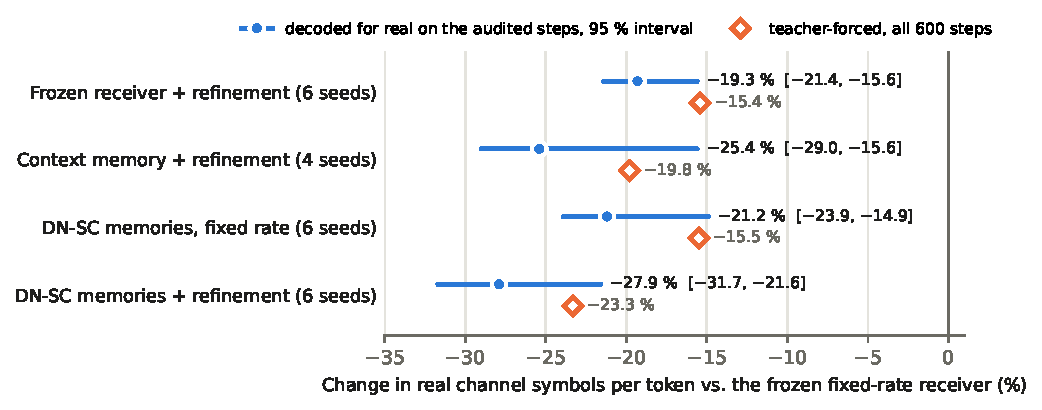
\includegraphics[width=\linewidth]{fig_primary_endpoint.pdf}
\caption{Change in real channel symbols per token for 90\,\% token accuracy
against the frozen fixed-rate receiver, return-link signalling of refinement
included. Dots: decoded for real on the audited steps with 95\,\% paired
bootstrap intervals; diamonds: teacher-forced on all 600 steps.}
\label{fig:primary}
\end{figure}

Table~\ref{tab:primary} and Fig.~\ref{fig:primary} give the primary endpoint.
With its memories and selective refinement, DN-SC reaches 90\,\% token
accuracy with 7.08 real channel symbols per token, against 9.23 for the frozen
fixed-rate receiver: a saving of 23.3\,\% with the return-link signalling
charged (28.3\,\% for the forward symbols alone, 20.7\,\% with an explicit
bitmap). The saving holds on every seed (between 10.5\,\% and 28.5\,\%;
$p = 0.031$, the smallest value six seeds allow). It holds on the three seeds
that had never been run before (20.6\,\% teacher-forced, 25.9\,\% decoded for
real). Decoded for real on the audited steps, the saving is 27.9\,\%
(95\,\% CI 21.6--31.7\,\%; 26.3\,\% with a bitmap). The real-decoding saving is
larger than the teacher-forced one because a fixed prefix suffers more from
error propagation than the refinement policy does.

\subsection{Where the saving comes from}
\label{sec:results-decomposition}

The receiver memories and selective refinement both contribute, and they
overlap. At a fixed rate, the memories of DN-SC alone save 15.5\,\%
teacher-forced (21.2\,\% decoded for real), with no return-link signalling at
all; the prior cross-entropy falls from 6.79 to 5.23 bits per token
(paired per-step difference $1.56$ [$1.41$, $1.72$] bits; $p = 0.031$).
Refinement alone saves the frozen receiver 15.4\,\% (19.3\,\% real; $p = 0.031$).
On top of the memories it adds a further 9.3\,\% teacher-forced (8.4\,\% real,
95\,\% CI 3.9--18.3\,\%). The better the receiver's prior, the less
uncertainty is left for refinement to resolve. The signalling is light: at the
operating threshold the requests cost 1.39 bits per token at their entropy
(1.52 as a bitmap), spread over 2.84 rounds per message, against 1.62 bits and
3.07 rounds for the frozen receiver.

The context memory, which needs no synchronisation, accounts for most of the
gain of the memories. On its four seeds it saves 19.8\,\% with refinement
(25.4\,\% real). Shipped adaptation (logit bias and LoRA slots, 24.2\,kbit per
adaptation step) lowers the prior by a further 0.37 bits per token
($[0.32, 0.41]$ per step; four seeds, $p = 0.125$, the floor for four seeds)
and the selective cost at the operating threshold by 0.12 symbols per token
($[0.10, 0.15]$).

\subsection{When shipping adaptation pays}
\label{sec:results-crossover}

Shipping the updates is not free. Charged at channel capacity, the 24.2\,kbit
per adaptation step pay for themselves against the frozen receiver only when
one update serves more than about 1{,}100 messages (forward symbols and
signalling), and against the context memory alone above about 6{,}100. In the
stream itself an update serves six messages, so for a single link the context
memory with refinement is the economical configuration. Shipped adaptation pays
where one update serves a cell or a multicast group.

\subsection{Limitations}
\label{sec:results-limitations}

\begin{itemize}
\item Six seeds give $p = 0.031$ for each of the two comparisons above
  (DN-SC and the frozen receiver with refinement, each against the frozen
  fixed-rate receiver). Corrected together with the context-memory comparison
  (Holm), the smallest adjusted value is 0.094. The context-memory receiver
  has four seeds, and its test cannot go below 0.125.
\item The frozen receiver's real-decoding gap ($+5.0$\,\%) sits at the 5\,\%
  limit of the decision rule; both measurements are reported.
\item One language model (GPT-2, 124M parameters) and one codebook. The
  temporal (news-chronology) stream was not repeated with the version 0.4
  decoder; with the earlier greedy decoder its real-decoding saving was
  21.1\,\% (two seeds).
\item Signalling and synchronisation are charged at channel capacity and
  assumed error-free; channel state and sentence length are assumed known at
  the receiver.
\item Seeds 0--2 and 3--5 ran on two different CPUs. Floating-point results
  differ in the last digits between machines; the code and the codebook are
  the same.
\end{itemize}

{\sloppy
\paragraph*{Data and code availability.}
The code, configurations, the decoder selection on validation text, and every
result file behind these tables (per-step logs included) are available at
\url{https://github.com/abraheemrashid99-sys/Wiley_paper} (branch
\texttt{review-fixes}, folder \texttt{results/gpt2\_v0.4\_six\_seeds}). The
command \texttt{python scripts/run\_quick.py} repeats the primary comparison on
a laptop CPU.\par}
